\begin{equation}
\dev{x}{t}=rx\left(1-\frac{x}{M}\right)-u \label{eq: ConstantHarvest}
\end{equation}
We introduce the following variable in order to simply calculations,
\begin{equation}
\beta=\frac{uM}{r}
\end{equation}
Solving the differential equation,
\begin{align*}
	\frac{\diff{x}}{rx\left(1-\frac{x}{M}\right)-u}&=\diff{t} \\
	\int_{x_0}^{x}\frac{\diff{\chi}}{r\chi\left(1-\frac{\chi}{M}\right)-u}&=\int_{0}^{t}\diff{\tau} \\
	\frac{M}{r}\int_{x_0}^{x}\frac{\diff{\chi}}{\chi\left(M-\chi\right)-\frac{Mu}{r}}&=t \\
	-\frac{M}{r}\int_{x_0}^{x}\frac{\diff{\chi}}{\chi^2-M\chi+\beta}&=t \nonumber
	\end{align*}
Finally, we model the above integral as one 
\begin{align}
	-\frac{M}{r}\int_{x_0}^{x}\frac{\diff{\chi}}{\left(\chi-\frac{M}{2}\right)^2-\frac{M^2}{4}+\beta}&=t
\end{align}
Consider $\alpha$ as follows,
\begin{equation}
	\alpha = \beta - \frac{M^2}{4} = rM\left(u-\frac{rM}{4}\right)
\end{equation}
We see that the sign of $\alpha$ determines the nature of the solutions. Then, if $u>rM/4$ implies $\alpha>0$,
\begin{align*}
\int_{x_0}^{x}\frac{\diff{\chi}}{\left(\chi-\frac{M}{2}\right)^2+\alpha}&=-\frac{r}{M}t \\
\frac{1}{\sqrt{\beta-\frac{M^2}{4}}}\left(\arctan\left(\frac{x-M/2}{\sqrt{\beta-M^2/4}}\right)-\arctan\left(\frac{x_0-M/2}{\sqrt{\beta-M^2/4}}\right)\right)&=-\frac{r}{M}t \\
\end{align*}
Therefore, for $\alpha > 0$ the population behaves as follows, 
\begin{align}
	x(t)=\frac{M}{2}+\sqrt{\beta-\frac{M^2}{4}} \tan \left(\arctan\left(\frac{x_0-M/2}{\sqrt{\beta-M^2/4}}\right)-\frac{r\sqrt{\beta-M^2/4}}{M}t\right) \label{eq: ConstantHarvest OverExploit}
\end{align}

Equation \ref{eq: ConstantHarvest OverExploit} show us that for some $t^*$, $x(t^*)=0$,independently of the initial condition $x_0$, since the argument inside the $\tan$ is monotone decreasing in $t$. 

If $u<rM/4$ implies $-\alpha>0$,
\begin{align*}
	\int_{x_0}^{x}\frac{\diff{\chi}}{\left(\chi-\frac{M}{2}\right)^2-(-\alpha)} &=-\frac{r}{M}t
\end{align*}
Considering the zeros of the denominator, $\lambda$ and $\overleftarrow{\lambda}$, 
\begin{equation}
	\begin{array}{cc}
	\lambda&=\frac{M}{2}+\sqrt{\frac{M^2}{4}-\beta} \\
	\overline{\lambda}&=\frac{M}{2}-\sqrt{\frac{M^2}{4}-\beta} \\
	\end{array}
\end{equation}
We can rewrite our expression as follows, 
\begin{align*}
\int_{x_0}^{x} \left(\frac{1}{\chi - \lambda}-\frac{1}{\chi - \overline{\lambda}}\right)\diff{\chi} &=-\frac{2r\sqrt{M^2/4-\beta}}{M}t \\
	\ln\abs{\frac{x - \lambda}{x - \overline{\lambda}}}&=\ln\abs{\frac{x_0- \lambda}{x_0 - \overline{\lambda}}}-\frac{2r\sqrt{M^2/4-\beta}}{M}t
\end{align*}
For simplifying calculations, we write, $\gamma=\frac{2r\sqrt{M^2/4-\beta}}{M}$. And we obtain as result,
\begin{align}
\frac{x - \lambda}{x - \overline{\lambda}} &=\frac{x_0- \lambda}{x_0- \overline{\lambda}}\mathrm e^{-\gamma t} \\
x-\lambda &=\left(x-\overline{\lambda}\right)\left(\frac{x_0- \lambda}{x_0- \overline{\lambda}}\right)\mathrm e^{-\gamma t}
\end{align}

For the sake of simplicity, consider $\xi=\frac{x_0-\lambda}{x_0-\overline{\lambda}}\mathrm{e}^{-\gamma t}$. Therefore,
\begin{align*}
	x\left(1-\xi\right)&=\lambda-\overline{\lambda}\xi\\
	x&=\frac{\lambda-\overline{\lambda}\xi}{1-\xi} \\	
	x&=\frac{\frac{M}{2}+\sqrt{\frac{M^2}{4}-\beta}-\left(\frac{M}{2}-\sqrt{\frac{M^2}{4}-\beta}\right)\xi}{1-\xi}\\
	x&=\frac{\frac{M}{2}+\sqrt{\frac{M^2}{4}-\beta}-\left(\frac{M}{2}-\sqrt{\frac{M^2}{4}-\beta}\right)\xi}{1-\xi}\\
	x&=\frac{\frac{M}{2}\left(1-\xi\right)+\sqrt{\frac{M^2}{4}-\beta}\left(1+\xi\right)}{1-\xi}\\
	x&=\frac{M}{2}+\sqrt{\frac{M^2}{4}-\beta}\frac{1+\xi}{1-\xi}
\end{align*}
Hence, for $-\alpha>0$, we have the following result,
\begin{align}
	x(t)&=\frac{M}{2}+\left(\sqrt{\frac{M^2}{4}-\beta}\right)\frac{\left(x_0-M/2\right)\left(1+\mathrm e^{-\gamma t}\right)-\sqrt{M^2/4-\beta}\left(1-\mathrm{e}^{-\gamma t}\right)}{\left(x_0-M/2\right)\left(1-\mathrm e^{-\gamma t}\right)+\sqrt{M^2/4-\beta}\left(1+\mathrm{e}^{-\gamma t}\right)} \label{eq: Time Expression for Harvest}
\end{align}

If $u=\frac{rM}{4}$, we solve equation \ref{eq: ConstantHarvest} as follows,
\begin{align}
-\frac{M}{r}\int_{x_0}^{x}\frac{d\chi}{\left(\chi-\frac{M}{2}\right)^2}&=t\\
\int_{x_0}^{x}\frac{d\chi}{\left(\chi-\frac{M}{2}\right)^2}&=-\frac{rt}{M}\\
\frac{1}{x-\frac{M}{2}}&=\frac{1}{x_0-\frac{M}{2}}-\frac{rt}{M}\\
\frac{1}{x-\frac{M}{2}}&=\frac{M-\left(x_0-\frac{M}{2}\right)rt}{M\left(x_0-\frac{M}{2}\right)} \\
x&=\frac{M}{2}+\frac{M\left(x_0-\frac{M}{2}\right)}{M-\left(x_0-\frac{M}{2}\right)rt} 
\end{align}

The results above stated can be explained directly from the equation \ref{eq: ConstantHarvest}, as we see in the graph \ref{fig: CriticalPoints},  $F(x,t)$ is a paraboloid, with its maximum at $F(x^*=M/2,t)=rM^2/4$.

When $u=0$, we have the regular logistic equation with critical points $x_{c_1}=0$ and $x_{c_2}=M$. With $x_{c_2}$ being an stable fixed point and $x_{c_1}$ an unstable fixed point. In general, these are the solutions to the equation $F(x,t)-u=0$,
\begin{equation}
x_{c_{2,1}}=\frac{M}{2}\pm \sqrt{\frac{M^2}{4}-u\frac{M}{r}}
\end{equation}

We observe that the critical points $x_c$, such that $\dev{x_c}{t}=F(x_c, t)-u=0$ are getting closer to each other, as $u$ is increasing; when $u=\frac{rM}{4}$ we only have one stable critical point. For $u> \frac{rM}{4}$, the population $x(t)$ has no real critical points and the derivative $\dev{x}{t}$ is always negative, implying, that we will lead always the population to extinction, extracting constantly at a rate greater than $\frac{rM}{4}$.

\begin{figure}[H]
	\centering
	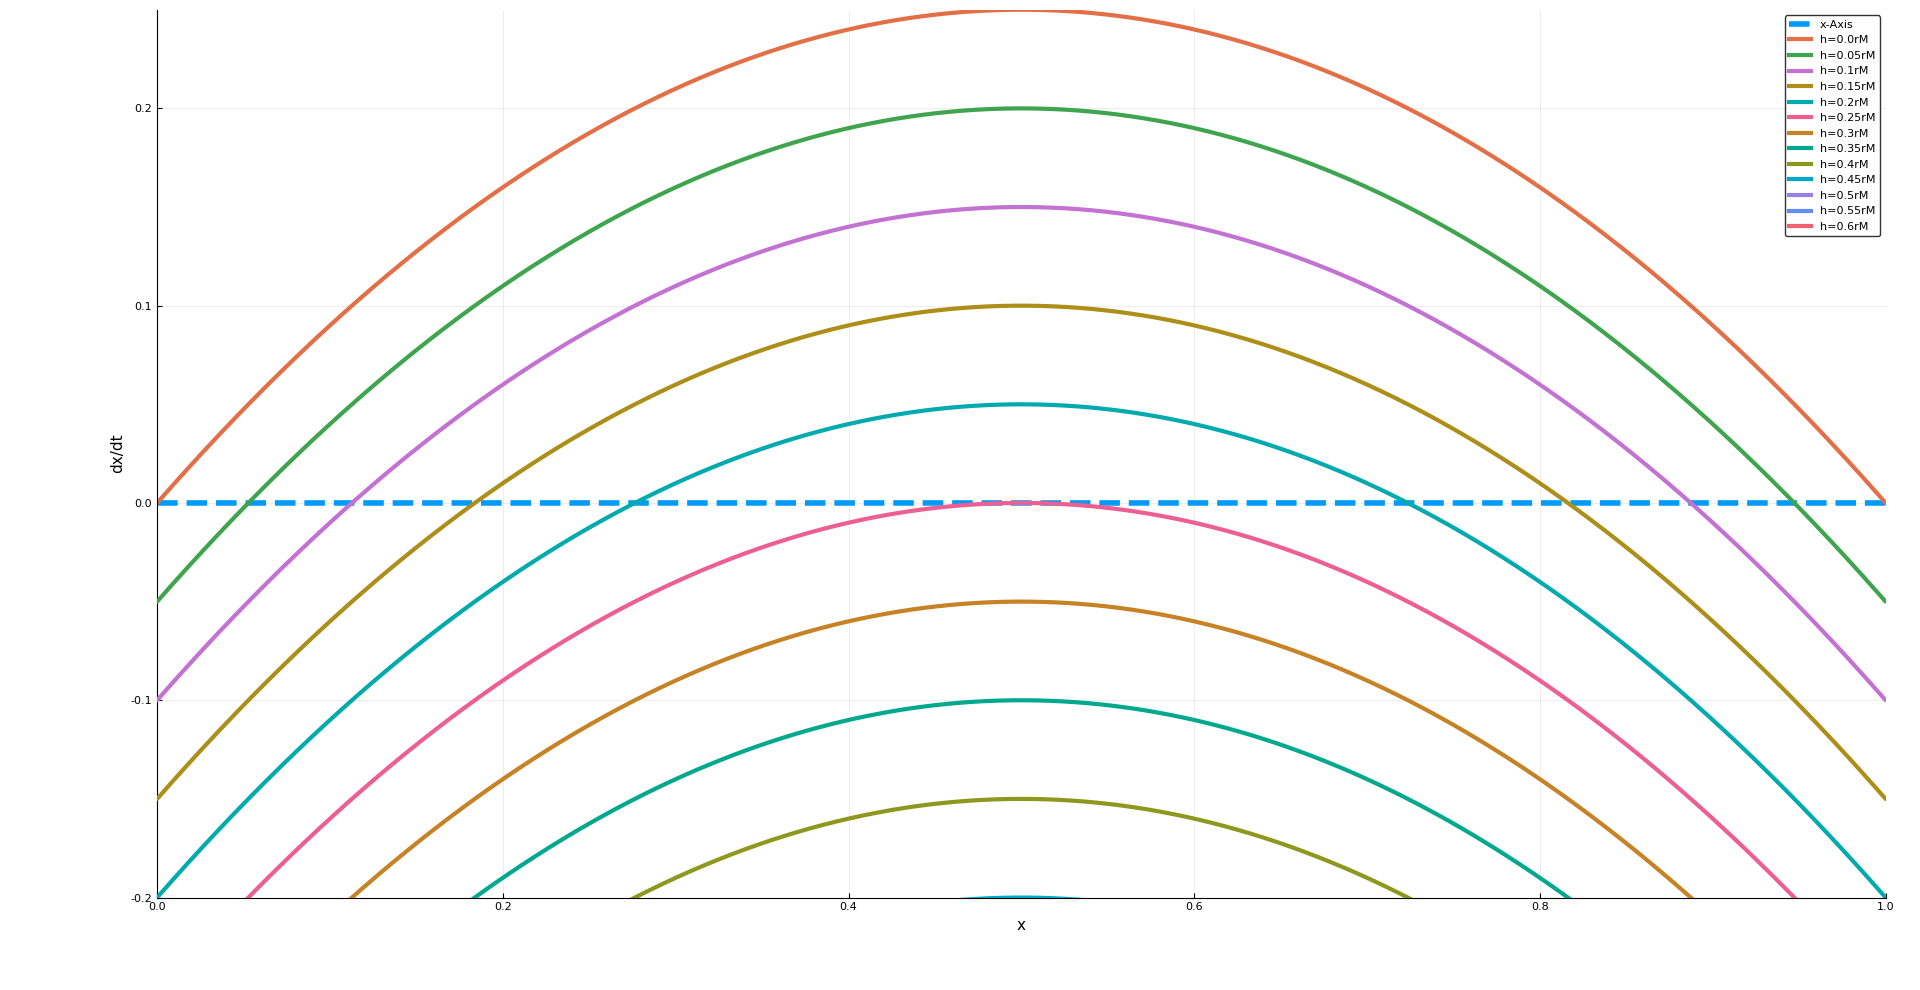
\includegraphics[width=0.8\textwidth]{CriticalPoints.png}
	\caption{Figure representing $\dev{x}{t}$ with different harvesting rates.}
	\label{fig: CriticalPoints}
\end{figure}
\begin{figure}
		\centering
		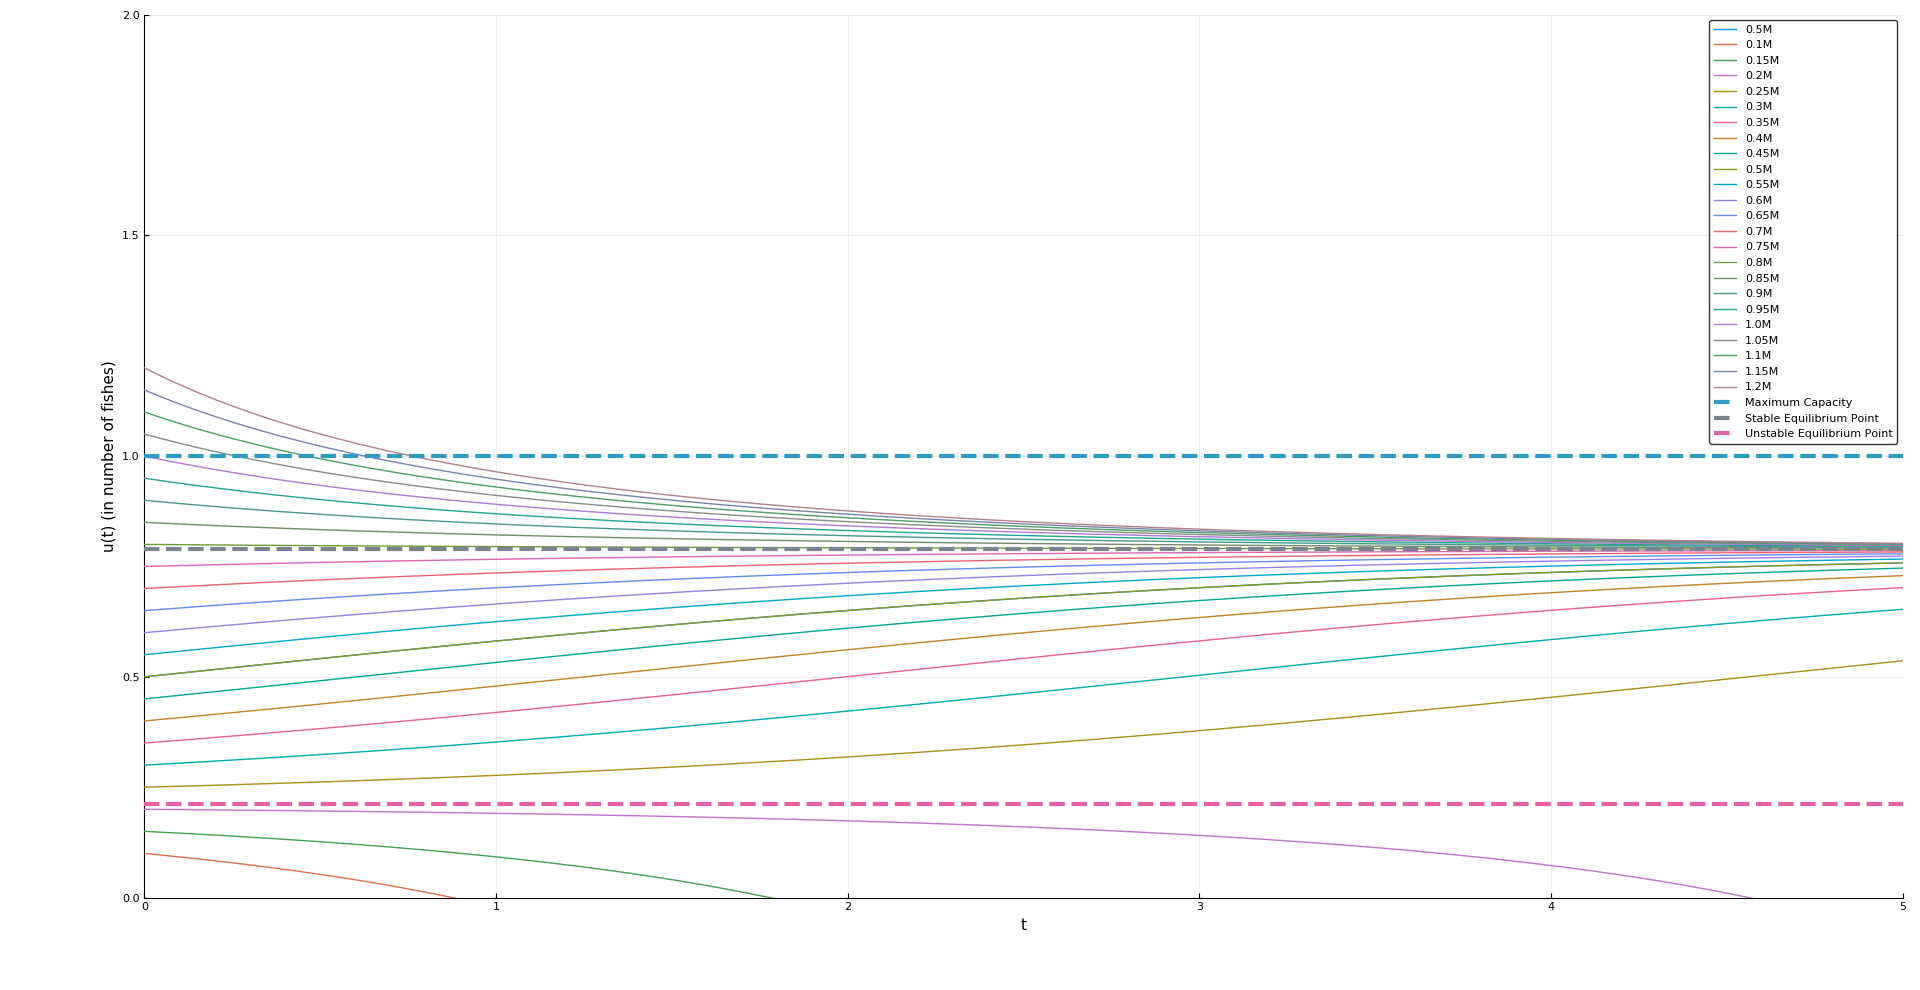
\includegraphics[width=0.8\textwidth]{SustainableConstant.png}
		\caption{Behavior for equation.}
		\label{fig: SustainableConstantHarvest}
\end{figure}
From the above analysis we have that,
\begin{equation}
0<u\leq\frac{rM}{4}
\end{equation}

